\documentclass[12pt]{article}
\usepackage[margin=1.5in]{geometry}
\usepackage{amsmath}
\usepackage{titling}
\usepackage{graphicx}
\usepackage{hyperref}
\usepackage{alphalph}
\usepackage{perpage}
\usepackage{amsmath}
\usepackage{amsfonts}
\usepackage{nameref}
\MakePerPage[1]{footnote}
\renewcommand{\thefootnote}{\alphalph{\value{footnote}}}

\setlength{\droptitle}{-2cm}

\pretitle{\begin{center}\Large}
\posttitle{\par\end{center}\vskip 0.5em}

\preauthor{\begin{center}\lineskip 2em}
\postauthor{\par\end{center}}

\predate{\begin{center}\normalsize}
\postdate{\par\end{center}}

\title{Task 1: Dynamic Time Warping Written Component}
\author{Kevin Yu \\ The University of Melbourne \\ Design of Algorithms (COMP20007)}
\date{\today}

\begin{document}
\maketitle

\section{Part B} \label{sec:partB}
\begin{itemize}
    \item Dynamic Time Warping (DTW) is an algorithm employed to measure the similarity between two sequences. It is particularly useful when two signals are of a different duration or are out of sync. Consider, for example, two signals representing the displacement of a foot and an arm during a walk. These signals are likely to be out of sync due to the natural coordination of human movement - it's often awkward to move one's arm and leg simultaneously. With DTW, one can allign these two signals, allowing us to find out which foot displacement corresponds to which arm displacement \cite{ref1}. This allows us to distinguish between individuals based on their unique walking styles. 
    \item With the signal discretised into a sequence of points, a naive way of measuring similariry would be taking an euclidean distance between the two signals. However, this simple sequence matching does not account for the fact that the two signals that may be dilated or out of sync (See Figure \ref{fig:dtw_vs_euc}). DTW solves this by seeking for the \textbf{temporal\footnote{process of adjusting the time axes of two signals so they align in time} alignment} that minimises the total distance between the two signals. 
    \item The cost matrix, $C \in \mathcal{M}_{n + 1, m + 1} \left(\mathbb{R}\right)$, is a $n+1 \times m+1$ matrix, where $n$ is the length of the first seququence ($x$) and $m$ is the length of the second sequence ($x'$). The matrix stores the \textbf{cumulative distance (cost)} between the two signals. The algorithm works by iteratively filling in the cost matrix, starting from the top-left corner all the way to the bottom-right corner. To initialise the matrix, we set $C_{0, 0} = 0$, and $C_{i, 0} = \infty$ and $C_{0, j} = \infty$ for $i, j > 0$. 
    \item The cost at, $C_{i, j}$, is determined by first calulating the distance of aligning the two signals at point $i, j$. Now, we add the minimum of the cost of aligning the two signals at the previous points - whether to insert a point ($C_{i - 1, j}$), delete a point ($C_{i, j-1}$), or match the two points ($C_{i - 1, j - 1}$).
\end{itemize}

\begin{figure}[h]
    \centering
    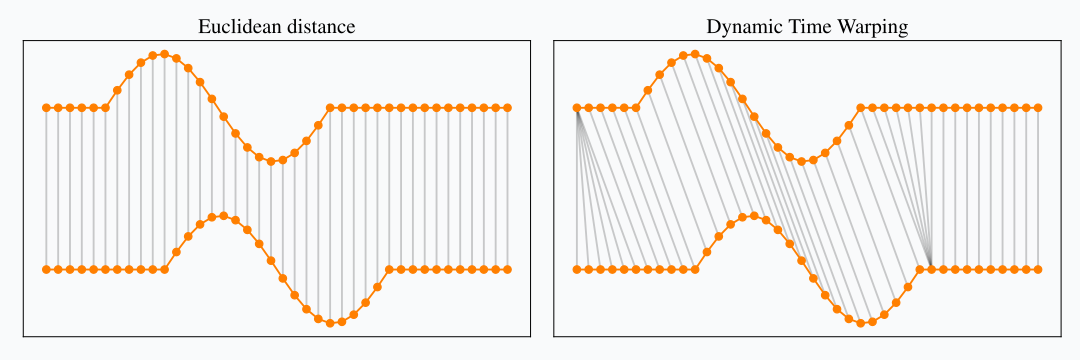
\includegraphics[width=1\textwidth]{images/dtw_vs_euc.png}
    \caption{Euclidean Distance vs DTW \cite{ref2}}
    \label{fig:dtw_vs_euc}
\end{figure}

\section{Part C}

Let $C(i, j)$ be the cost of an optimal alignment of the two sequences $x$ and $x'$ up to the $i$th and $j$th points, respectively. With the process of calculating the optimal path outlined in \nameref{sec:partB}, it leads to the following recurrence:

$$
    C(i, j) = |x_i - x'_j| + \min \begin{cases}
    C(i - 1, j), \; \; \; \; \, \text{  (insertion)}\\
    C(i, j - 1), \; \; \; \; \, \text{  (deletion)}\\
    C(i-1, j-1) \text{  (match)}
    \end{cases}, \;\; \text{for } i, j > 0
$$
It is convenient to define the initial conditions as follows:
$$
    C(0, 0) = 0, \;\; C(i, 0) = \infty \text{ for } i > 0, \;\; C(0, j) = \infty \text{ for } j > 0.
$$


Now, with the recurrence relation set up, we can solve the problem using bottom-up approach. We should first solve the subproblems with smaller indices before moving on to the larger indices as the cost of aligning the two signals at point $i, j$ depends on the cost of aligning the two signals at the previous points. Therefore, We start by filling in the cost matrix $C$ from the top-left corner to the bottom-right corner. The final DTW cost is the value of $C_{n, m}$.

\section{Part E}
Whilst the computaional complexity of Part A is $\Theta(nm)$, the computational complexity of Part D is $\Theta(nw)$, where $w$ is the boundary constraint or the window size. The window size is a constraint that limits the alignment path to a window around the diagonal. This is clear from this relation:

$$
C_{i, j} = \sum_{i = 1}^{n}{\sum_{j = i - w \geq 1}^{i + w \leq m}{|x_i - x'_j| + \min \begin{cases}
C_{i - 1, j}, \, \, \text{   (insertion)}\\
C_{i, j-1}, \, \, \text{   (deletion)}\\
C_{i-1, j-1} \text{  (match)}
\end{cases}}} 
$$

\section{Part G - 1 mark}
The computational complexity of Part F with total length constraint is $\Theta(nmp)$, where $p$ is the maximum \textbf{p}ath length constraint. The maximum path length constraint is a constraint that limits the alignment path to a path of length at most $p$. \\

Let $D_{i, j, k}$ be the cost of the optimal alignment of the first $i$ elements of $x$ and the first $j$ elements of $x'$ with a path length of $k$. The relation for this problem is as follows:

$$
D_{i, j, k} = \sum_{k = 1}^{p}{\sum_{i = 1}^{n}{\sum_{j = 1}^{m}{|x_i - x'_j| + \min \begin{cases}
D_{i-1, j, k-1} \, \, \; \, \text{   (insertion)}\\
D_{i, j-1, k-1} \, \, \; \, \text{   (deletion)}\\
D_{i-1, j-1, j-1} \text{  (match)}
\end{cases}}}} 
$$


\begin{thebibliography}{9}
\bibitem{ref1} 
Olsen, N. L., Markussen, B., \& Raket, L. L. (2018). Simultaneous inference for misaligned multivariate functional data. Journal of the Royal Statistical Society: Series C, 67(5), 1147-1176. https://doi.org/10.1111/rssc.12276

\bibitem{ref2}
Tavenard, R. (2021). An introduction to Dynamic Time Warping. Retrieved from https://rtavenar.github.io/blog/dtw.html
\end{thebibliography}

\end{document}